\subsubsection{\stid{4.01} \dataviz\ Software Development Kits} 

\paragraph{\textbf{DataViz SDK Overview}}
\paragraph{}

The Data \& Visualization (DataViz) SDK aims to create a production-quality infrastructure necessary to manage, share, and facilitate data analysis of mission-critical codes at scale. The project focuses on community development and a commitment to success via quality improvement policies, better build and deployment processes, and the ability to use diverse, independently developed DataViz SDK projects, in combination, for data analysis and visualization problems.

The DataViz SDK's responsibility is to coordinate the disparate documentation, development, testing, deployment activities, and develop the necessary tooling and shared infrastructure to serve these goals. This coordination's resulting product is a unified set of usable, standardized, and interoperable packages ready for the upcoming exascale machines. We have designed the efforts to support the DataViz SDK to fit within the overarching goal to leverage and integrate data management, analysis, and visualization techniques developed across the ECP ST ecosystem to support scientific discovery and understanding.

In addition, DataViz SDK provides a capability supporting collaborative analysis and visualization software development, helping independent teams accelerate the adoption of best practices, enabling interoperability of independently developed software, and improving developer productivity and sustainability of the software products.

\paragraph{\textbf{Key Challenges}}
\paragraph{}

Scientists and engineers from various research cultures and significantly different software engineering maturity levels develop Data \& Visualization software packages. In addition to the challenges outlined in Section~\ref{subsubsect:ecosystem-sdk}, ECP Data \& Visualization software packages will use different combinations of dependency software in various configurations. Visualization applications and libraries, in particular, utilize lower-level graphics libraries from an OpenGL stack needing reliably mapped to a diverse set of underlying hardware.  These applications demand the deployment infrastructure support the appropriate combination of software and hardware-based rendering on NVIDIA, AMD, or Intel GPUs and accelerated offscreen rendering APIs like EGL.  Requirements such as these place the DataViz SDK between the hardware teams and the analysis and visualization software developers preparing to run on new architectures yet delivered by ECP.

DataViz SDK software packages also have, on average, a much deeper dependency chain than is typical within HPC.  As of this writing, an optimized set of twelve ECP DataViz SDK packages requires over 160 dependencies.  Many packages share these dependencies, each with their own set of constraints.  This combination presents a unique challenge to ensure compatibility, interoperability, and reliability of the entire stack as a whole, beyond the individual packages.

\paragraph{\textbf{Solution Strategy}}
\paragraph{}

First, the DataViz SDK solution strategy involves pursuing usability, standardization, interoperability, and sustainability goals through a set of community policies to improve software practices. The DataViz SDK community policy tasks have required us to define a common terminology for effective communication.

Second, we leverage shared infrastructure, such as the Spack~\cite{gamblin+:sc15} package manager and CI testing at ECP facilities. We built the SDK release and delivery deployment goals on Spack as a unifying package manager, while our reliability and sustainability goals benefit from and leverage the facilities' CI testing infrastructure. 

Finally, we define a set of spack meta-packages, ecp-vis-sdk and ecp-io-sdk, to enable the delivery of ECP targeted configurations of data and visualization packages through E4S.  These meta-packages establish dependencies for the packages within the DataViz SDK, and serve as the backbone of our interoperability testing and deployment efforts. 

\begin{itemize}
\item ecp-vis-sdk includes data analysis and visualization packages such as ASCENT, Catalyst, Cinema, ParaView, VTK-m along with data reduction and compression libraries like SZ, and ZFP.
\item ecp-io-sdk includes input and output (I/O) services like ADIOS, Darshan, hdf5, parallel-netcdf, unifyfs, and veloc.
 \end{itemize}

\noindent
The packages contained in the two meta-packages represent software at different maturity and readiness for release. The early release strategy was to push product readiness for inclusion in the E4S releases by assisting packages with Spack packaging and CI testing. We will continue to evolve the maturity level and interoperability of the packages while preparing for subsequent releases.

\paragraph{\textbf{Recent Progress}}
\paragraph{}

In pursuit of establishing a baseline set of software quality across the entire ECP ST area, the SDK projects have been collectively developing a set of community policies a given package must adhere to be an E4S member package.  These community policies cover areas including publicly accessible documentation, mandatory spack packaging, testing practices, and other policy areas.  The DataViz SDK has played an active role in this panel by proposing new policies, refining language on official policies, and soliciting community feedback.  We are nearing a final set of initial guidelines required by the E4S project for packages to be accepted as a first-class E4S Member Package.  These community policies intended to be an ongoing collaborative effort to elevate the standard of software quality, reliability, and sustainability for the entire ECP software ecosystem.

In addition, recent progress included the completion of the following three milestones during the fiscal year 2020.

\textit{STDV01-06} --- Improved CI capabilities. During this milestone, we worked to ensure that all of the packages within the DataViz SDK were utilizing Continuous Integration in some way as part of their development workflow and software process. While the packages span a wide range of maturity and robustness of the software process, they all have incorporated at least a baseline CI capability (some far more extensive than others). Most leverage a public cloud CI like Travis or GitHub Actions, while others rely on internal resources from an internal GitLab or BitBucket ser er. We also improved the spack packaging for several of the SDK projects and integrated the remaining projects into the SDK meta-packages.

\textit{STDV01-08} --- HDF Virtual Object Layer Architecture (VOL) documentation and ECP HPC-CI integration. During this time, we worked directly within the ADIOS and VTK-m projects to enable the newly developed ECP HPC-CPI capability. These two projects served as early adopters of the Gitlab-CI environment running directly on HPC resources at ORNL. The SDK coordinated directly with ORNL facilities personnel to debug the CI environment worked to identify issues other Data \& Viz projects are likely to encounter, and develop the initial capability for ADIOS and VTK-m. From this work, the SDK can assist other data and visualization projects in implementing the ECP HPC CI capability through both guidance and best practice recommendation and direct technical development assistance.

\textit{STDV01-14} --- Optimized Spack configurations and CI. The default configuration of most spack packages is intended to produce the most compatible version, but not necessarily the most optimal for large scale HPC. In particular, packages may have key features disabled by default essential to HPC, such as MPI support and FORTRAN language bindings. The two meta-packages were enhanced to ensure that an optimized configuration explicitly targets ECP target platforms for every direct data and visualization package dependency.

\paragraph{\textbf{Next Steps}}
\paragraph{}

We highlight our next steps in the follow on project milestones.

\textit{STDV01-17} --- Cross SDK CI testing. The focus of this release is to demonstrate successful interoperable CI testing. The DataViz SDK is building out a CI infrastructure to allow all ST products within the Data \& Visualization focus area to be regularly built and tested with each other to ensure interoperability. This milestone is to have the CI system running with as many ST products in the DataViz SDK successfully building together, satisfying each other's dependencies.

\textit{STDV01-29} --- Hardening to ensure SENSEI is deployable and reliable at scale. Establishing Spack recipes for the SENSEI software coupled with the hardening of the in transit code-base will go a long way in mitigating the risks associated with availability and defects for ECP applications. 

\paragraph{HDF5}
\paragraph{Overview}
\paragraph{}
HDF5 is a data model, I/O library, and file format to store and manage data. It supports an unlimited variety of datatypes, and is designed for flexible and efficient I/O for high volume and complex data. Its extensive ecosystem is illustrated by over 2,000 repositories on GitHub depending on HDF5 or 160 packages in Spack along with many third-party tools that support HDF5, e.g., MATLAB, and open source packages, e.g., h5py, Pandas, Keras, and TensorFlow. 

HDF5 is portable and is extensible, allowing applications to evolve in their use of HDF5. It supports many different types of data stores, such as local, clustered, and networked file systems and object stores. HDF5 is highly customizable through its purposefully designed extension interfaces, Virtual Object Layer (VOL) and Virtual File Driver (VFD) interfaces as shown in Figure~\ref{fig:HDF5-Arch}.
\begin{figure}[htb]
    \centering
    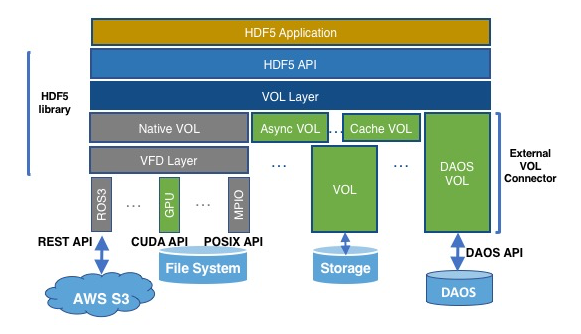
\includegraphics[width=0.75\textwidth]{projects/2.3.4-DataViz/2.3.4.01-DataViz-SDK/HDF5-Arch-small.png}
    \caption{\label{fig:HDF5-Arch}
    HDF5 architecture: green rectangles represent dynamically loaded VFD and VOL connectors to access data on different storage devices; grey and blue rectangles represent components of the HDF5 library.}
\end{figure}

 The most recent extensions include support for Intel DAOS high-performance storage and NVidia’s GPUDirect interface for data movement between storage and GPU memory. 
Numerous ECP applications use HDF5 or high-level libraries built on top of HDF5 (for example, H5Part) for data management. Therefore, HDF5 is a critical part of the Data \& Vis SDK. 

The HDF Group team’s responsibility is to maintain HDF5 on the ECP systems, develop enhancements to boost the performance of the ECP HDF5 applications; integrate enhancements developed by other ECP teams (e.g. DataLib, ExaIO); and deliver HDF5  to the ECP users as a part of the Spack package and Data \& Vis SDK. 

\paragraph{Key  Challenges}
\paragraph{}

The HDF Group team faces two major challenges. The first challenge is extending HDF5 legacy software to deliver high-performing features for the Exascale systems while maintaining HDF5 current performance standards and avoiding HDF5 software disruption for the millions of non-HPC users. The second challenge is the complexity of the HDF5 software that may lead to its misapplication, resulting in poor performance, especially in the HPC environment. The third challenge is delivering contributions to HDF5 created by other teams promptly and according to HDF5 regression testing and coding standards.

\paragraph{Solution Strategy}
\paragraph{}
To lower the barrier for adopting HDF5 by ECP applications and delivering new features timely, The HDF Group (1) provides HDF5 software that is regularly tested on and released for ECP platforms, (2) integrates newly developed features into mainstream HDF5 and makes them promptly available via Spack and Data \& Vis SDK, (3) educates HDF5 users on the best HDF5 practices and new features, and (4) works closely with ECP teams on features development and applications’ tuning. 

\paragraph{Recent Progress}
\paragraph{}
In 2021, The HDF Group developers made enhancements to the HDF5 library to address requirements of the HDF5 ExaIO VOL connectors - \href{https://github.com/hpc-io/vol-async}{Async}, \href{https://github.com/hpc-io/vol-external-passthrough}{Pass-through} and \href{https://github.com/hpc-io/vol-cache}{Cache} VOL connectors, and \href{https://github.com/hpc-io/vfd-gds}{NVIDIA GPU Direct I/O VFD}. The requested changes are available in the \href{https://github.com/HDFGroup/hdf5}{HDF5 develop branch} on GitHub and will be released in the HDF5 1.13 series of releases and later. The releases can be obtained from The HDF Group \href{https://portal.hdfgroup.org/display/support/Downloads}{website} or using the Spack package manager.  

We performed a major refactoring of internal HDF5 library APIs to accommodate new \href{https://portal.hdfgroup.org/display/HDF5/Asynchronous+operations+with+HDF5+VOL+connectors}{asynchronous APIs}.  New HDF5 APIs are designed for HDF5 VOL connectors that support asynchronous operations using the \href{https://portal.hdfgroup.org/display/HDF5/Event+Set}{HDF5 Event Set APIs}. This feature allows I/O to proceed in the background while the application performs other tasks. 

HDF5 VOL and VFD APIs were reworked to address the issues brought up by the ExaIO developers. We held a webinar on the changes to help HDF5 VOLs and VFDs developers with porting existing connectors to the new version of the HDF5 library. Recording and slides are available from \href{https://www.hdfgroup.org/2021/09/webinar-followup-new-features-in-the-hdf5-1-13-0-release/}{The HDF Group website}. 
ECP ExaIO VOL connectors were integrated with Spack. The HDF Group also worked with the ExaIO team on coordination of the HDF5 library and VOL connectors releases.

CI testing was set up to keep HDF5 VOL connectors development and the HDF5 library development in sync. During our integration and testing work, we addressed several issues and desired improvements reported by the DataLib and ExaIO teams. We added a feature that allows auto-detection of a VOL connector used to open an HDF5 file; the feature is available in HDF5 1.13.0 and HDF5 1.12.2 and later maintenance releases; we made improvements to collective metadata write operations and addressed the issues found when using IBM SpectrumScale MPI on the Summit system.

The required changes to the HDF5 library architecture for supporting HDF5 VOL connectors added 7-10\% overhead for the applications that do not use connectors at all. The overhead was especially prominent for applications that work with a lot of HDF5 objects. We identified and implemented several optimizations and saw up to 10\% reduction in time spent by a \href{https://jira.hdfgroup.org/browse/HDFFV-9671}{benchmark} provided to us by LLNL. 

Other integration work includes support for SZ and ZFP compression filters in the maintenance releases of the HDF5 library starting with the HDF5 1.10.7 release. The HDF Group developers also investigated HDF5 performance with SZ and ZFP HDF5 compression filters. Our study showed that HDF5 filters pipeline implementation doesn't create additional overhead for SZ and ZFP compressions.

In 2021, The HDF Group continued with \href{https://www.hdfgroup.org/category/hdf5-resources-for-ecp-users/}{outreach activities}. Recent activities included two Tutorials \href{https://www.hdfgroup.org/2021/05/webinar-followup-hdf5-application-tuning-there-is-more-than-one-way-to-skin-a-catfish-part-2/} {"HDF5 Application Tuning"} and \href{https://www.hdfgroup.org/2021/09/webinar-followup-new-features-in-the-hdf5-1-13-0-release}{"New features in HDF5 1.13.0"}, and a \href{https://portal.hdfgroup.org/pages/viewpage.action?pageId=73924784}{white paper}. The HDF team delivered HDF5 tutorial for ECP 2021 annual meeting and gave a talk on the new ECP VOL/VFD features at the HDF5 BoF at the annual meeting.


\paragraph{Next Steps}
\paragraph{}
The HDF Group activities will continue in two areas:  productization of the HDF5 features developed for ECP applications and outreach. In 2022, we will continue with CI testing on ECP systems and will provide maintenance releases of the HDF5 library.  We will deliver a TOOLKIT for the VOL connectors developers to facilitate the development of new HDF5 connectors. We will integrate HDF5 subfiling VFD and multi-dataset feature (access data in multiple datasets using a single I/O call) that we are developing under the ExaIO project and release it in the mainstream HDF5. We will continue working with the ECP HDF5 applications teams on I/O performance, conduct Tutorials and Webinars, and create additional documentation on efficient usage of HDF5 in the ECP HPC environment. 
